\section{Trace and fleet evaluation}\label{sec:trace}

A design chosen at one operating point is operated on a load that varies. Two simulator tools bound the fuel of a design on a load trace, and
neither needs part-load efficiency curves that the model does not have. Both are simulator-only: no trace-based result is a prediction of a fuel bill.

\paragraph{Ideal part-load bound.}
A load trace is split into quantile bins of IT power. The design is evaluated at the median load and coolant temperatures of each bin (and the ambient
temperature when the trace has it), and the fuel is weighted by the time in the bin. The plant is re-sized to every bin, so efficiency does not depend on load: this is ideal
part-load and a lower bound on fuel within the model. Bins in which the design is infeasible are reported by time share and excluded from the energy.

\paragraph{Modular gensets.}
To remove the ideal assumption without inventing efficiency curves, the prime mover is split into $n$ identical units that run at rated output or not at all. The installed capacity is
the largest bin need times a margin, the units online in a bin are the smallest number that covers its need, the plant is solved with that output, and the surplus electricity is curtailed,
so its fuel is wasted. The modularity penalty is the fuel above the ideal part-load bound. Because fuel scales with generation for both prime movers, the penalty depends on the shape of the
load trace and on the unit count and, to first order, not on the technology; parasitic loads that do not scale with generation, such as electric chillers or a heat pump, break the tie slightly.
Not modeled are unit efficiency depending on unit size, minimum run time, start-up and ramp limits, capacity limits of heat-recovery equipment and chillers, and standby units beyond the capacity margin.

\paragraph{A synthetic example.}
\Cref{fig:fig_part_load} applies both tools to a synthetic trace of \val{pl.n_samples} samples (IT load drawn from a normal distribution with a mean of 24~MW and a standard deviation of 5~MW, clipped to 8 to 30~MW, \val{pl.bins} bins, seed 0). It is not Frontier data. For
a turbine plant with absorption cooling and a wet tower at a chilled fraction of 0.5, the ideal bound is \val{pl.turbine.ideal_mwh}~MWh of fuel and a single unit burns \val{pl.turbine.fuel1_mwh}~MWh. The modularity penalty is
\val{pl.turbine.u1_pct}\% for one unit and \val{pl.turbine.u2_pct}\% for two, then \val{pl.turbine.u3_pct}\% for three, \val{pl.turbine.u4_pct}\% for four, \val{pl.turbine.u6_pct}\% for six,
\val{pl.turbine.u8_pct}\% for eight and \val{pl.turbine.u12_pct}\% for twelve units; the values for the engine plant are the same. That the one-unit and two-unit penalties coincide and that the engine and the turbine coincide are properties of this trace and of the
scaling argument above, not findings about the technologies. With one sample trace and one design, the figure shows the size of the effect that a fleet of more units can recover in the model; it makes no statement about real units.

\begin{figure}[tbp]
\centering
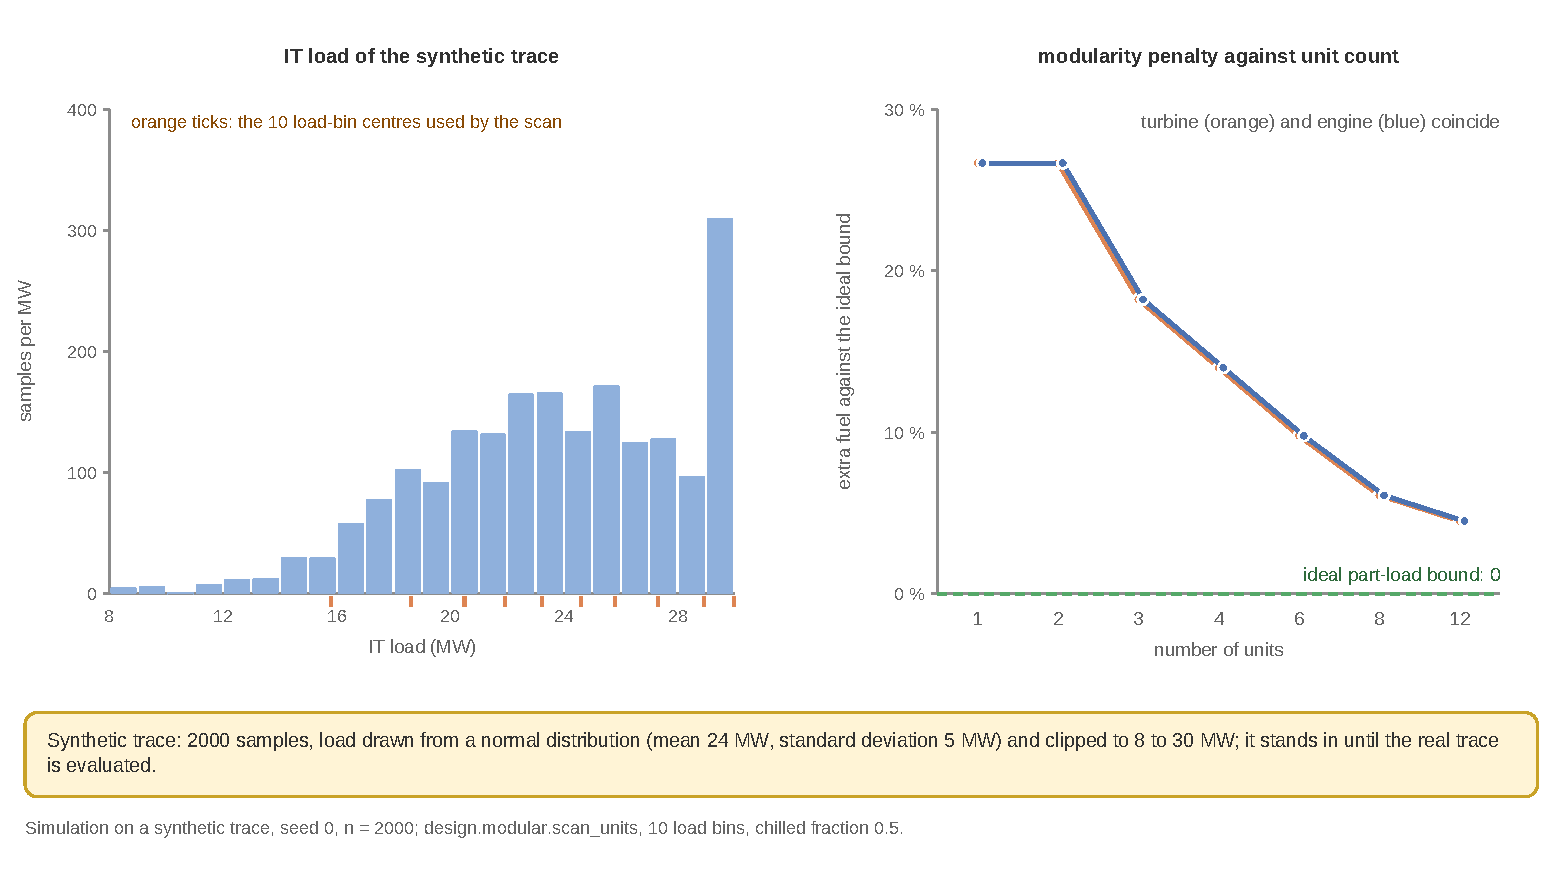
\includegraphics[width=\linewidth]{figures/pdf/fig_part_load.pdf}
\caption{Part-load behavior on a \textbf{synthetic} trace (not Frontier data; \val{pl.n_samples} samples, seed 0, simulation): load histogram with the bin centers used (left) and modularity penalty against the number of
units with the ideal bound at zero (right), for turbine and engine plants with absorption cooling and a wet tower. The trace stays synthetic until the real trace is evaluated. Data: \texttt{assets/part\_load.json}.}
\label{fig:fig_part_load}
\end{figure}

\paragraph{Frontier trace.}
The loader for the published Frontier energy dataset maps explicit columns, and the file has not been downloaded. The evaluation of the catalog and of modular fleets on the measured trace is therefore pending:
\todo{Frontier trace results}.
